%%%%%%%%%%%%%%%%%%%%%%%%%%%%%%%%%%%%%%%%%
% Short Sectioned Assignment
% LaTeX Template
% Version 1.0 (5/5/12)
%
% This template has been downloaded from:
% http://www.LaTeXTemplates.com
%
% Original author:
% Frits Wenneker (http://www.howtotex.com)
%
% License:
% CC BY-NC-SA 3.0 (http://creativecommons.org/licenses/by-nc-sa/3.0/)
%
%%%%%%%%%%%%%%%%%%%%%%%%%%%%%%%%%%%%%%%%%

%----------------------------------------------------------------------------------------
%	PACKAGES AND OTHER DOCUMENT CONFIGURATIONS
%----------------------------------------------------------------------------------------

\documentclass[paper=a4, fontsize=11pt]{scrartcl} % A4 paper and 11pt font size
\usepackage[margin=0.7in]{geometry}
\usepackage[T1]{fontenc} % Use 8-bit encoding that has 256 glyphs
\usepackage{fourier} % Use the Adobe Utopia font for the document - comment this line to return to the LaTeX default
\usepackage[english]{babel} % English language/hyphenation
\usepackage{amsmath,amsfonts,amsthm} % Math packages

\usepackage{lipsum} % Used for inserting dummy 'Lorem ipsum' text into the template

\usepackage{sectsty} % Allows customizing section commands
\allsectionsfont{\bfseries\sffamily\scshape} % Make all sections centered, the default font and small caps

\usepackage{fancyhdr} % Custom headers and footers
\pagestyle{fancyplain} % Makes all pages in the document conform to the custom headers and footers
\fancyhead{} % No page header - if you want one, create it in the same way as the footers below
\fancyfoot[L]{} % Empty left footer
\fancyfoot[C]{} % Empty center footer
\fancyfoot[R]{\thepage} % Page numbering for right footer
\renewcommand{\headrulewidth}{0pt} % Remove header underlines
\renewcommand{\footrulewidth}{0pt} % Remove footer underlines
\setlength{\headheight}{13.6pt} % Customize the height of the header

\numberwithin{equation}{section} % Number equations within sections (i.e. 1.1, 1.2, 2.1, 2.2 instead of 1, 2, 3, 4)
\numberwithin{figure}{section} % Number figures within sections (i.e. 1.1, 1.2, 2.1, 2.2 instead of 1, 2, 3, 4)
\numberwithin{table}{section} % Number tables within sections (i.e. 1.1, 1.2, 2.1, 2.2 instead of 1, 2, 3, 4)

\setlength\parindent{0pt} % Removes all indentation from paragraphs - comment this line for an assignment with lots of text

\usepackage[english]{babel}
\usepackage{graphicx}

%----------------------------------------------------------------------------------------
%	TITLE SECTION
%----------------------------------------------------------------------------------------

\newcommand{\horrule}[1]{\rule{\linewidth}{#1}} % Create horizontal rule command with 1 argument of height

\title{	
\normalfont \normalsize 
\textsc{University of Southern California, Computer Science} \\ [25pt] % Your university, school and/or department name(s)
\horrule{0.5pt} \\[0.4cm] % Thin top horizontal rule
\huge Machine Learning: HomeWork 2 \\ % The assignment title
\horrule{2pt} \\[0.5cm] % Thick bottom horizontal rule
}

\author{Rohit Kondekar\\
740-581-9473} % Your name

\date{\normalsize\today} % Today's date or a custom date
\allowdisplaybreaks
\begin{document}

\maketitle % Print the title


%----------------------------------------------------------------------------------------
%	PROBLEM 1
%----------------------------------------------------------------------------------------
\section{Question 1}
\subsection{Regression with heterogenous noise}


\begingroup
Solution a:\\
As the noise is independently distributed but donot have to be identically distributed, This implies the presence of either heteroscedasticity, or correlations i.e. the covariance matrix \begin{math}\Sigma\end{math} may be a diagonal matrix.\\

As noise is normally distributed with \begin{math}~N(0,\sigma_{n}^{2})\end{math}:

\begin{align*} 
P(\varepsilon_{n}) &= (2\Pi)^{\dfrac{-n}{2}}|\Sigma|^{\dfrac{-1}{2}}exp(\dfrac{-1}{2}\varepsilon_{n}\Sigma^{-2}\varepsilon_{n})
\end{align*}

As they are independently distributed - 
\begin{align*}
L(\varepsilon) = \prod_{i=1}^{n}P(\varepsilon_{n}) &= (2\Pi)^{\dfrac{-n^{2}}{2}}|\Sigma|^{\dfrac{-n}{2}}exp(\dfrac{-1}{2}\sum_{i=1}^{n}[(y_{i}-x_{i}^{T}\beta)^{T}\Sigma^{-1}(y_{i}-x_{i}^{T}\beta)])\\
l(\varepsilon) &= log(L)\\
l(\varepsilon) &=  const - \dfrac{n}{2}log(|\Sigma|) - \dfrac{1}{2}\sum_{i=1}^{n}[(y_{i}-x_{i}^{T}\beta)^{T}\Sigma^{-1}(y_{i}-x_{i}^{T}\beta)]
\end{align*}


Solution b:
\begin{align*}
\hat{\beta} &= argmin_{b}(Y-X\beta)\Sigma^{-1}(Y-X\beta)\\
&= (Y^{T}-\beta^{T}X^{T})\Sigma^{-1}(Y-X\beta)\\
&= (Y^{T}\Sigma^{-1}-\beta^{T}X^{T}\Sigma^{-1})(Y-X\beta)\\
&= Y^{T}\Sigma^{-1}Y - \beta^{T}X^{T}\Sigma^{-1}Y - Y^{T}\Sigma^{-1}X\beta + \beta^{T}X^{T}\Sigma^{-1}X\beta
\end{align*}

Properties used:
\begin{align*}
\nabla_{\Theta}(b^{T}\Theta) &= b\\
\nabla_{\Theta}(\Theta^{T}A\Theta) &= (A + A^{T})\Theta
\end{align*}

\begin{align*}
\dfrac{dl(\varepsilon)}{d\beta} &= -2(X^{T}\Sigma^{-1}Y) + [X^{T}\Sigma^{-1}X + (X^{T}\Sigma^{-1}X)^{-1}]\beta = 0\\\\
2X^{T}\Sigma^{-1}X\beta &= 2X^{T}\Sigma^{-1}Y\\
\beta &= (X^{T}\Sigma^{-1}X)^{-1}X^{T}\Sigma^{-1}Y
\end{align*}

As \begin{math}X^{T}\Sigma^{-1}X\end{math} is a symmetric matrix.
\endgroup

\subsection{Smooth Coefficients}
\begingroup
Solution a:\\
To define this regularizer, a special constant matrix C p$\times$p is defined such that $C_{ij}=1$ whenever $i=j$, $C_{ij}=0$ when $j=n$ and $C_{ij}=-1$ when $j-i=1$. For eg. if $\beta$ is $4\times1$ then :

\begin{align*}
C &= 
\begin{bmatrix}
1 & -1 & 0 & 0\\
0 & 1 & -1 & 0\\
0 & 0 & 1 & -1\\
0 & 0 & 0 & 0
\end{bmatrix}\\
C\beta &= 
\begin{bmatrix}
\beta_{1}-\beta_{2}\\
\beta_{2}-\beta_{3}\\
\beta_{3}-\beta_{4}\\
0\\
\end{bmatrix}
\end{align*}

Therefore the new regularized equation can be stated as:
\begin{align*}
RSS(\beta) &= \dfrac{1}{2}\sum_{i=1}^{m}(y_{i}-\theta^{T}x_{i})^{2} + \lambda_{1}||C\beta||_{2}^{2} + \lambda_{2}||\beta||_{2}^{2}\\
&= \dfrac{1}{2}(Y-\beta X)^{T}(Y-\beta^{T} X) + \lambda_{1}(C\beta)^{T}(C\beta) + \lambda_{2}\beta^{T} \beta
\end{align*}

Solution b:\\
\begin{align*}
\hat{\beta} &= argmin_{b} \dfrac{1}{2}(Y-\beta X)^{T}(Y-\beta^{T} X) + \lambda_{1}\beta^{T} C^{T}C\beta + \lambda_{2}\beta^{T}\beta\\
\dfrac{dRSS(\beta)}{d\beta} &= 0\\
0 &= X^{T}X\beta - X^{T}Y + \lambda_{1}[C^{T}C + C^{T}C]\beta + \lambda_{2}\beta\\
X^{T}X\beta + 2\lambda_{1}C^{T}C\beta + \lambda_{2}\beta &= X^{T}Y\\
\beta &= (X^{T}X + 2\lambda_{1}C^{T}C + \lambda_{2}I)^{-1}X^{T}Y
\end{align*}
\endgroup


\subsection{Linearly Constrained Linear Regression}
\begingroup
Solution:\\
This problem can be solved using langrange multiplier by adding $\lambda (A\beta - b)$ as it has a non-empty set of solutions.\\
Also, originally without this constraint $\hat{\beta}$ was given by:
\begin{align}
\hat{\beta} &= (X^{T}X)^{-1}X^{T}Y
\end{align}
Now with the given constraint we have to minimize :
\begin{align}
\hat{\beta}^{'} &= argmin_{\beta} \dfrac{1}{2}(Y-\beta^{T}X)^{T}(Y-\beta^{T}X) + \lambda(A\beta -b)
\end{align}
Where $\hat{\beta}^{'}$ is the constrained Maximum likelihood estimator. With constraint : $A\beta - b = 0$\\

Therefore differentiating the equation we get:
\begin{align}
X^{T}X\beta - X^{T}Y + A^{T}\lambda &= 0\\
A\beta - b &= 0
\end{align}

To estimate $\lambda$ : multiplying minimizing Eq. by $A(X^{T}X)^{-1}$ we get:\\
\begin{align*}
A(X^{T}X)^{-1}X^{T}X\beta  - A(X^{T}X)^{-1}X^{T}Y + A(X^{T}X)^{-1}A^{T}\lambda &= 0\\
A\beta - A\hat{\beta} + A(X^{T}X)^{-1}A^{T}\lambda &= 0\\
A(X^{T}X)^{-1}A^{T}\lambda &= A\hat{\beta} - b\\
\end{align*}
\begin{align}
\lambda &= (A(X^{T}X)^{-1}A^{T})^{-1}(A\hat{\beta} - b)
\end{align}

Now solving for $\beta$:
\begin{align}
X^{T}X\beta &= X^{T}Y - A^{T}[A(X^{T}X)^{-1}A^{T})^{-1}(A\hat{\beta} - b)]\\
\beta &= (X^{T}X)^{-1}(X^{T}Y - A^{T}[A(X^{T}X)^{-1}A^{T})^{-1}(A\hat{\beta} - b)])
\end{align}
\endgroup




%----------------------------------------------------------------------------------------
%	PROBLEM 2
%----------------------------------------------------------------------------------------
\section{Question: Online Learning}
Solution:
As we know that whenever perceptron correctly classifies a datapoint: $y_{n}W_{i}x_{n}>0$ else when incorrectly classifies $y_{n}W_{i}x_{n}<=0$.\\
Therefore our optimization equation boils down to solving [Assumnig L2norm squared]:

\begin{align*}
%\intertext{minimize}
\text{Minimize~~} \dfrac{1}{2}||w_{i+1}-w_{i}||^{2}_{2}\\
\text{With constraint~~} y_{n}(w_{i+1}x_{n})>0
\end{align*}

Therefore writing it in terms of lagrange operator:
\begin{align*}
\text{Minimize~~} \dfrac{1}{2}(w_{i+1}-w_{i})^{T}(w_{i+1}-w_{i}) + \lambda [y_{n}(w_{i+1}x_{n})]\\
\text{Minimize~~} \dfrac{1}{2}w_{i+1}^{T}w_{i+1} - w_{i+1}^{T}w_{i} + \lambda[y_{n}w_{i+1}x_{n}]
\end{align*}
Taking Derivative:
\begin{align*}
-w_{i+1} - w_{i} + \lambda y_{n}x_{n} &= 0\\
w_{i+1} &= w_{i} - \lambda y_{n}x_{n}
\end{align*}

To obtain the value of lambda differentiate the minimizing equation wrt lambda. We get:

\begin{align*}
y_{n}w_{i+1}x_{n} = 0
\end{align*}
Substituting $w_{i+1}$ from last equation:
\begin{align*}
y_{n}[w_{i} - \lambda y_{n}x_{n}]x_{n}&=0\\
\lambda &= \dfrac{y_{n}w_{i}x_{n}}{x_{n}^{2}}
\end{align*}



%----------------------------------------------------------------------------------------
%	PROBLEM 3
%----------------------------------------------------------------------------------------
\section{Question: Kernels}

\subsection{}
Solution a:\\
We can show that, K3 is indeed a positive definite kernal function if :\\\\
$X^{T}(a_{1}K_{1}+a_{2}K_{2})X >= 0$\\\\
It can be written as: \\\\
$a_{1}X^{T}K_{1}X+X^{T}a_{2}K_{2})X >= 0$\\\\

As $X^{T}K_{1}X>=0$ and $X^{T}K_{2}X>=0$ as K1 and K2 are PSDs and $a_{1}>=0$,$a_{2}>=0$ which shows that: \\\\

$a_{1}X^{T}K_{1}X+X^{T}a_{2}K_{2})X >= 0$\\\\

Therefore it is Positive SemiDefinite Matrix.\\\\

Solution b:\\
Any matrix of the form:

\begin{align*}
K_{3} = 
\begin{bmatrix}
f(x_{1})f(x_{2}) & f(x_{1})f(x_{2}) & ... & f(x_{1})f(x_{n})\\
... & ... & ... & ...\\
f(x_{n})f(x_{1}) & f(x_{n})f(x_{2}) & ... & f(x_{n})f(x_{n})\\
\end{bmatrix}
\end{align*}


Can be broken down to: $ FF^{T} $ where
\begin{align*}
F = 
\begin{bmatrix}
f(x_{1})\\
f(x_{2})\\
.\\
.\\
f(x_{n})\\
\end{bmatrix}
\end{align*}

So We have to show that $X^{T}FF^{T}X >=0$ 

\begin{align*}
X^{T}FF^{T}X &= (F^{T}X)^{T}F^{T}X\\
&= || F^{T}X ||_{2}^{2}\\
|| F^{T}X ||_{2}^{2} &>=0\\
X^{T}FF^{T}X &>= 0
\end{align*}


Solution c:\\
This is bascically the Hadamard product of two positive semidefinite matrices, which is always positive definite. We can show that using Eigen Value Decomposition.\\\\

Let K1 = $\sum\mu_{i}k1_{i}k1_{i}^{T}$ and K2 = $\sum\nu{i}k2_{i}k2_{i}^{T}$
\begin{align*}
K1 \circ K2 &= \sum\mu_{i}k1_{i}k1_{i}^{T} \circ \sum\nu{j}k2_{j}k2_{j}^{T}\\
&= \sum_{ij}\mu_{i}\nu{j}(k1_{i} \circ k2_{j})(k1_{i} \circ k2_{j})^{T}
\end{align*}

To show that $(k1_{i} \circ k2_{j})(k1_{i} \circ k2_{j})^{T}$ is positive:

\begin{align*}
X(k1_{i} \circ k2_{j})(k1_{i} \circ k2_{j})^{T}X &= (\sum_{k}k1_{i,k}k2_{j,k}x_{k})^{2} \geq 0
\end{align*}
This shows that it is positive definite matrix.
%----------------------------------------------------------------------------------------
%	PROBLEM 4
%----------------------------------------------------------------------------------------
\section{Question: Bias-Variance Tradeoff}




%----------------------------------------------------------------------------------------
%	PROBLEM 5
%----------------------------------------------------------------------------------------
\section{Question: Programming Assignment}

\begin{large}
***Please Note: \\
\textbf{Log taken is Natural Log: Matlabs Log() function.}
\end{large}\\\\

\textbf{(1) top 3 words that occur most frequently?}\\

{ (enron,600) (will,351) (please,291) }\\\\

\textbf{(2)Updating equation for w and b for batch gradient descent}\\

Without Regularization:
\begin{align*}
\text{Repeat \{}\\
w_{j}^{t+1} &= w_{j}^{t} - \eta[\sum_{i=1}^{m}(h(x^{i}) - y^{i})x_{j}]\\
b^{t+1} &= b^{t} - \eta \sum_{i=1}^{m}(h(x^{i}) - y^{i})\\
\text{\}}
\end{align*}
In Matlab this can be written as:\\\\
weights = weights + $\eta$*((y-hypothesis)'*x)';\\
b = b + $\eta$*(sum(y-hypothesis));\\\\
\textbf{Note: Here h(x) is a sigmoid function.}\\\\
With Regularization:
\begin{align*}
\text{Repeat \{}\\
w_{j}^{t+1} &= w_{j}^{t} - \eta[\sum_{i=1}^{m}(h(x^{i} - y^{i})x_{j} - \lambda w_{j}^{t})]\\
b^{t+1} &= b^{t} - \eta \sum_{i=1}^{m}(h(x^{i}) - y^{i})\\
\text{\}}
\end{align*}
In Matlab this can be written as:\\\\
weights = weights + $\eta$*((y-hypothesis)'*x+lambda*w')';\\
b = b + $\eta$*(sum(y-hypothesis));\\

\textbf{Note: Here h(x) is a sigmoid function.}\\\\

\textbf{(3)(b)}
\begin{tabular}{l*{5}{c}}
L2 norm without regularization	& 0.001 & 0.01 & 0.05 & 0.1 & 0.5\\
\hline
EmailSpam & 2.5903 & 7.7726 & 26.4429 & 51.2757 & 253.4047\\
Ionosphere & 1.5111 & 4.7440 & 19.1862 & 39.9547 & 189.6151\\
\end{tabular}\\\\

\textbf{(4)(b)}
\begin{tabular}{l*{11}{c}}
L2 norm $\eta=0.01$	& 0 & 0.05 & 0.1 & 0.15 & 0.2 & 0.25 & 0.30 & 0.35 & 0.4 & 0.45 & 0.50 \\
\hline
EmailSpam & 2.602 & 2.596 & 2.590 & 2.584 & 2.578 & 2.572 & 2.565 & 2.559 & 2.553 & 2.547 & 2.541\\
Ionosphere & 1.501 & 1.498 & 1.495 & 1.492 & 1.489 & 1.486 & 1.483 & 1.480 & 1.477 & 1.475 & 1.472
\end{tabular}\\



\textbf{(5)Updating equation for w and b for Newton's method}\\\\
In Newton's Method the basic update equation is given by:\\\\

\textbf{Without Regularization}
\begin{align*}
w^{t+1} \leftarrow w^{t} - (H^{t})^{-1}\bigtriangledown\varepsilon(w^{t})
\end{align*}

Where $H^{t}$ is given by:
\begin{align*}
\text{For Weights}~~~ H(w^{t}_{j}) &= \sum_{i=1}^{m}(h(x^{i})(1-h(x^{i})x^{i}_{j}(x^{i}_{j})^{T}))\\
\text{For Bias}~~~ H &= \sum_{i=1}^{m}(h(x^{i})(1-h(x^{i}))\\
\end{align*}

And $\bigtriangledown\varepsilon(w^{t})$ is given by:
\begin{align*}
\text{For Weights}~~~ \bigtriangledown\varepsilon(w^{t}_{j}) &= \sum_{i=1}^{m}(h(x^{i}) - y^{i})x^{i}_{j}\\
\text{For Bias}~~~ 
\bigtriangledown\varepsilon(b) &= \sum_{i=1}^{m}(h(x^{i}) - y^{i})
\end{align*}

In Matlab this can be achieved by:\\\\
(x' * (hypothesis-y)) * (x' * diag(hypothesis) * diag(1-hypothesis) * x)\\\\

\textbf{With Regularization:}
\begin{align*}
w^{t+1} \leftarrow w^{t} - (H^{t})^{-1}\bigtriangledown\varepsilon(w^{t})
\end{align*}

Where $H^{t}$ is given by:
\begin{align*}
\text{For Weights}~~~ H(w^{t}_{j}) &= \sum_{i=1}^{m}(h(x^{i})(1-h(x^{i})x^{i}_{j}(x^{i}_{j})^{T}))+ 2\lambda diag(1)\\
\text{For Bias}~~~ H &= \sum_{i=1}^{m}(h(x^{i})(1-h(x^{i})) \\
\end{align*}

And $\bigtriangledown\varepsilon(w^{t})$ is given by:
\begin{align*}
\text{For Weights}~~~ \bigtriangledown\varepsilon(w^{t}_{j}) &= \sum_{i=1}^{m}(h(x^{i}) - y^{i})x^{i}_{j} + 2\lambda w_{j}\\
\text{For Bias}~~~ 
\bigtriangledown\varepsilon(b) &= \sum_{i=1}^{m}(h(x^{i}) - y^{i})
\end{align*}

\textbf{(6b) L2 norm of w for EmailData = }4.0437e+33\\
\textbf{(6b) L2 norm of w for IonoData = }Infinity (NaN)\\\\


\textbf{(7)(b)}
\begin{tabular}{l*{11}{c}}
L2 norm Newtons	& 0 & 0.05 & 0.1 & 0.15 & 0.2 & 0.25 & 0.30 & 0.35 & 0.4 & 0.45 & 0.50 \\
\hline
EmailSpam & 4e+33 & 12.5 & 10.39 & 9.25 & 8.482 & 7.91 & 7.462 & 7.09 & 6.78 & 6.52 & 6.29\\
Ionosphere & NaN & 16.006 & 12.227 & 10.454 & 9.362 & 8.600 & 8.029 & 7.578 & 7.210 & 6.900 & 6.635
\end{tabular}\\

Note: Column 1 with lambda = 0 gives value for unregularized version.\\\\


\textbf{(7)(c): Cross Entropy value after 50 iterations for regularized at different lambdas and unregularized }\\\\
\begin{tabular}{l*{11}{c}}
CrossEntropy 50 Steps	& 0 & 0.05 & 0.1 & 0.15 & 0.2 & 0.25 & 0.30 & 0.35 & 0.4 & 0.45 & 0.50 \\
\hline
EmailSpam & NaN & 15.76 & 23.0 & 28.33 & 32.65 & 36.32 & 39.55 & 42.43 & 45.05 & 47.46 & 49.69\\
Ionosphere & NaN & 7.79 & 10.80 & 12.87 & 14.49 & 15.81 & 16.95 & 17.94 & 18.82 & 19.61 & 20.33
\end{tabular}\\\\


\textbf{(8) Explanation for result in 3 and 4}\\
For Email and Ionosphere data, in case of unregularized we can see that, as step size size increases there are more spikes (zig-zag) but it still manages to converge (get lower cross-entropies) to some point. For lower step sizes the curve is much more smoother but the change in cross-entropy is much lower between subsequent steps.\\\\
In Case of regularized version, the cross entropy achieved by the end is much higher for higher regularizers because the model is more simpler. Also the model is not able to converge at higher step sizes for regularized version, and shows a zigzag nature, in gradient descent. This suggests that, larger the regularization, smaller the step size should be.\\

\textbf{(9) Explanation for result in 4 and 7}\\
From results, we can see that, Newton's method converges faster (in 4-5 iterations here) as compared to gradient descent. But it is slower computationaly as it has to compute the inverse of Hessian Matrix. For many dimensions, this would be significantly slower. So for higher dimension, it is better to use gradient descent, but for lower dimensions, Newton's method is much more faster.



\newpage
%Figures


\begin{figure}[h!]
  \caption{Cross-Entropy wrt Steps: Email Train Data Unregularized}
  \centering
    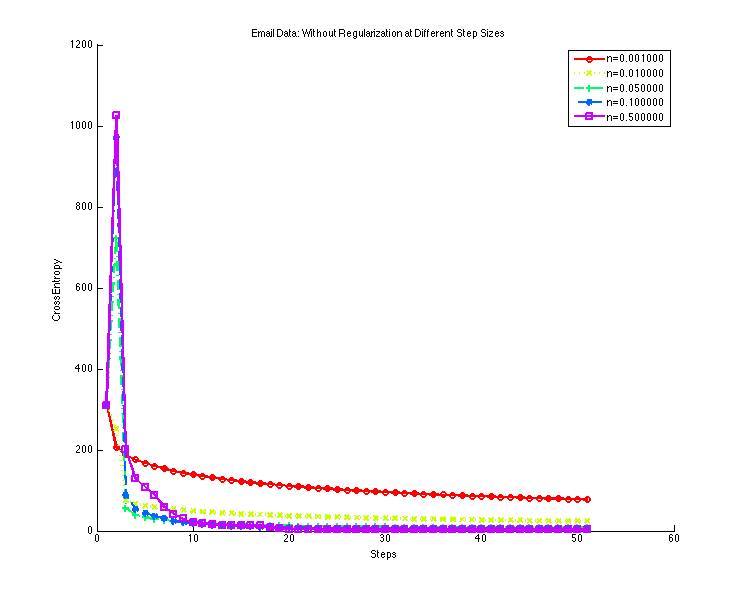
\includegraphics[width=0.8\textwidth]{../Pics/Fig1_email_unreg.png}
\end{figure}


\begin{figure}[h!]
  \caption{Cross-Entropy wrt Steps: Ionosphere Train Data Unregularized}
  \centering
    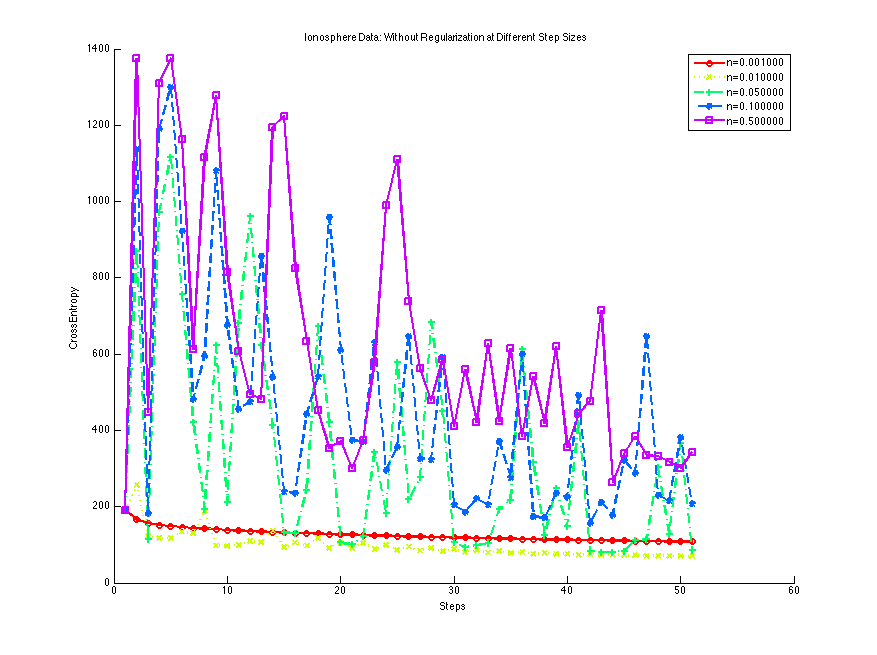
\includegraphics[width=0.8\textwidth]{../Pics/Fig2_iono_unreg.png}
\end{figure}


\begin{figure}[h!]
  \caption{Cross-Entropy wrt Steps: Email Train Data Regularized}
  \centering
    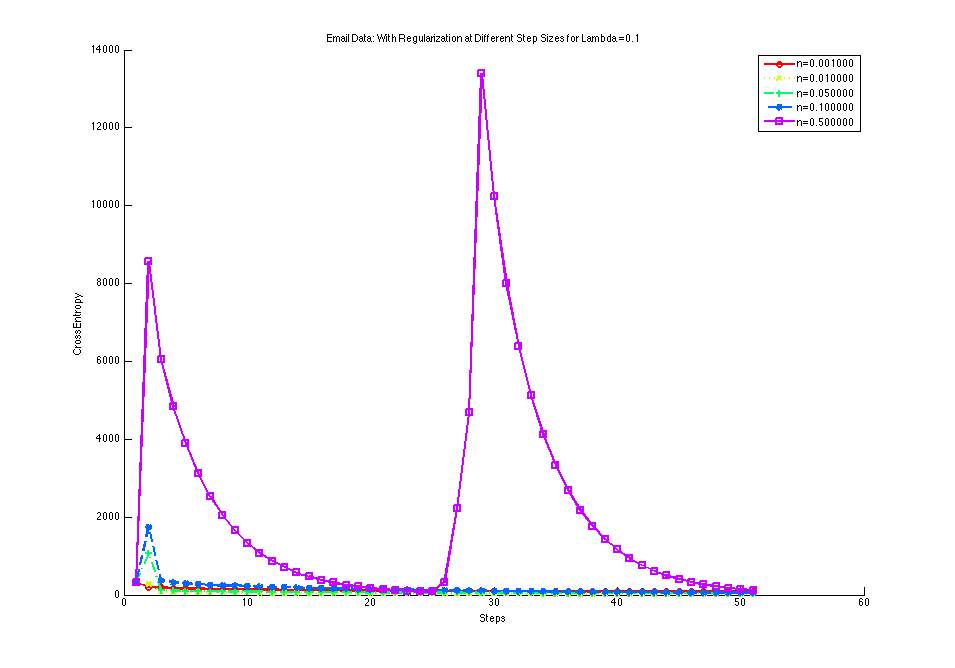
\includegraphics[width=0.8\textwidth]{../Pics/Fig3_email_reg.png}
\end{figure}

\begin{figure}[h!]
  \caption{Cross-Entropy wrt Steps: Ionosphere Train Data Regularized}
  \centering
    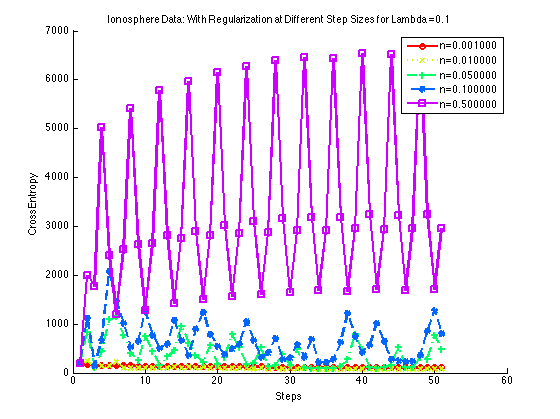
\includegraphics[width=0.8\textwidth]{../Pics/Fig4_iono_reg.png}
\end{figure}

\begin{figure}[h!]
  \caption{Cross-Entropy vs Regularizing Coefficients: Email: Step Size = 0.001}
  \centering
    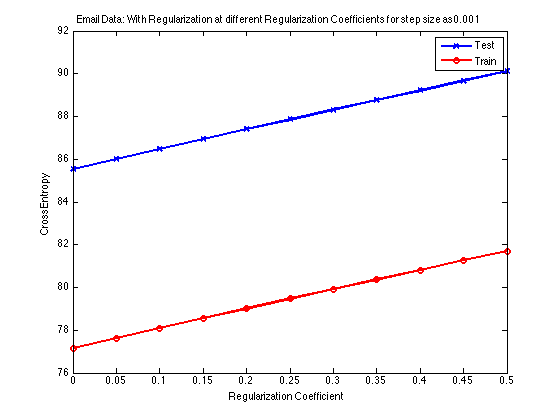
\includegraphics[width=0.8\textwidth]{../Pics/subGraphsEmail/Fig1.png}
\end{figure}

\begin{figure}[h!]
  \caption{Cross-Entropy vs Regularizing Coefficients: Email: Step Size = 0.01}
  \centering
    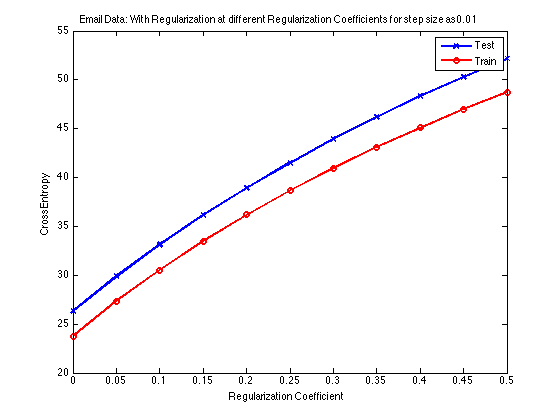
\includegraphics[width=0.8\textwidth]{../Pics/subGraphsEmail/Fig2.png}
\end{figure}

\begin{figure}[h!]
  \caption{Cross-Entropy vs Regularizing Coefficients: Email: Step Size = 0.05}
  \centering
    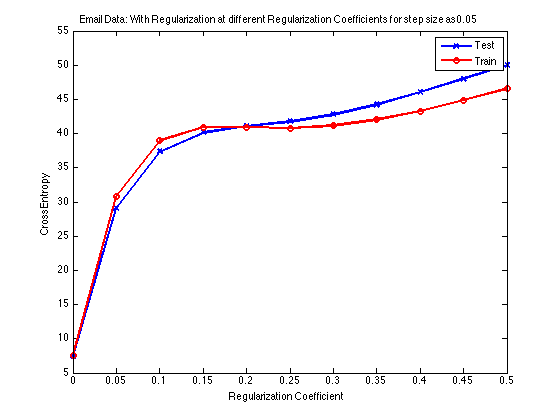
\includegraphics[width=0.8\textwidth]{../Pics/subGraphsEmail/Fig3.png}
\end{figure}

\begin{figure}[h!]
  \caption{Cross-Entropy vs Regularizing Coefficients: Email: Step Size = 0.1}
  \centering
    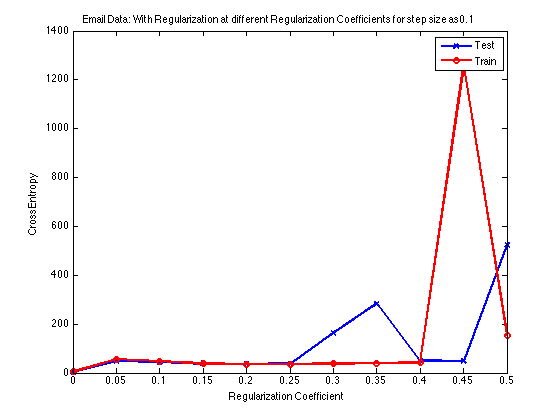
\includegraphics[width=0.8\textwidth]{../Pics/subGraphsEmail/Fig4.png}
\end{figure}

\begin{figure}[h!]
  \caption{Cross-Entropy vs Regularizing Coefficients: Email: Step Size = 0.5}
  \centering
    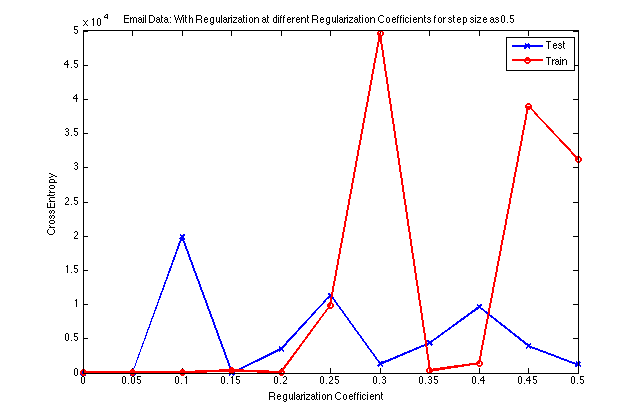
\includegraphics[width=0.8\textwidth]{../Pics/subGraphsEmail/Fig5.png}
\end{figure}


% Iono data
\begin{figure}[h!]
  \caption{Cross-Entropy vs Regularizing Coefficients: Ionosphere: Step Size = 0.001}
  \centering
    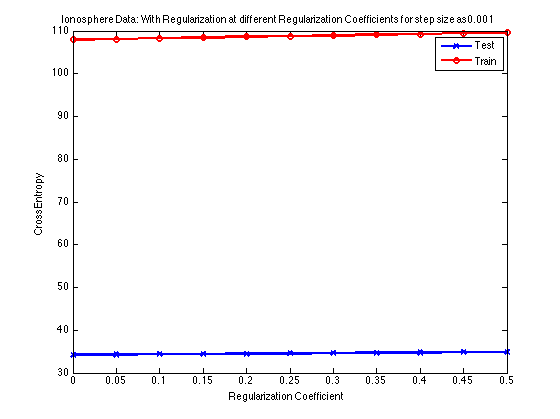
\includegraphics[width=0.8\textwidth]{../Pics/subGraphIono/Fig1.png}
\end{figure}

\begin{figure}[h!]
  \caption{Cross-Entropy vs Regularizing Coefficients: Ionosphere: Step Size = 0.01}
  \centering
    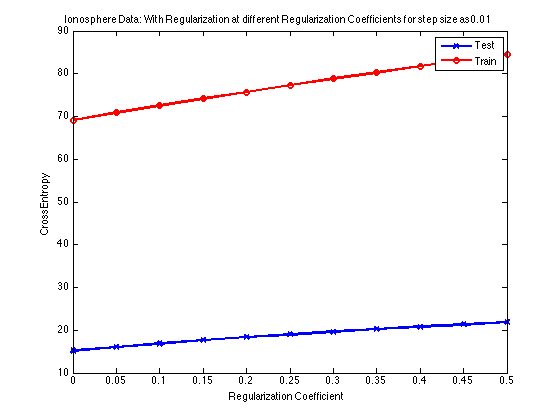
\includegraphics[width=0.8\textwidth]{../Pics/subGraphIono/Fig2.png}
\end{figure}

\begin{figure}[h!]
  \caption{Cross-Entropy vs Regularizing Coefficients: Ionosphere: Step Size = 0.05}
  \centering
    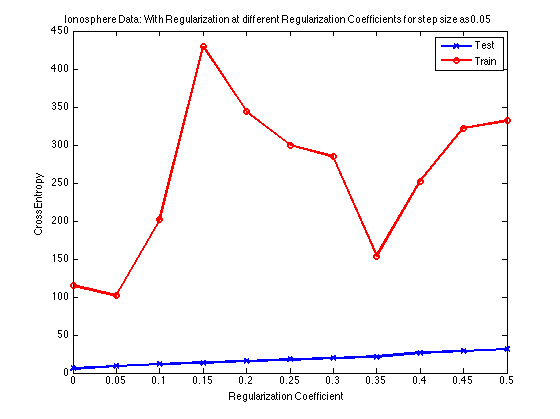
\includegraphics[width=0.8\textwidth]{../Pics/subGraphIono/Fig3.png}
\end{figure}

\begin{figure}[h!]
  \caption{Cross-Entropy vs Regularizing Coefficients: Ionosphere: Step Size = 0.1}
  \centering
    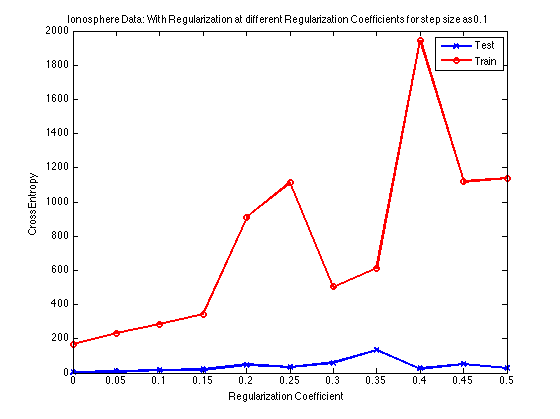
\includegraphics[width=0.8\textwidth]{../Pics/subGraphIono/Fig4.png}
\end{figure}

\begin{figure}[h!]
  \caption{Cross-Entropy vs Regularizing Coefficients: Ionosphere: Step Size = 0.5}
  \centering
    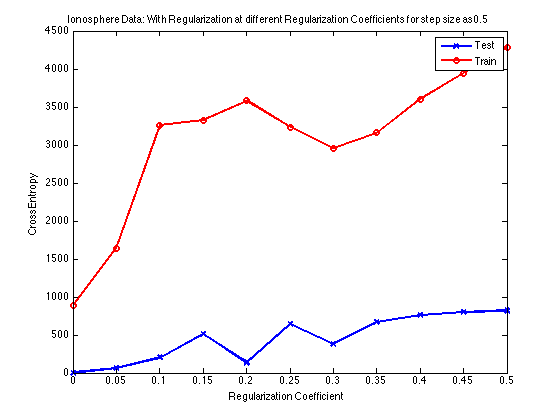
\includegraphics[width=0.8\textwidth]{../Pics/subGraphIono/Fig5.png}
\end{figure}



\begin{figure}[h!]
  \caption{Cross-Entropy wrt Steps: Email Train Data Unregularized}
  \centering
    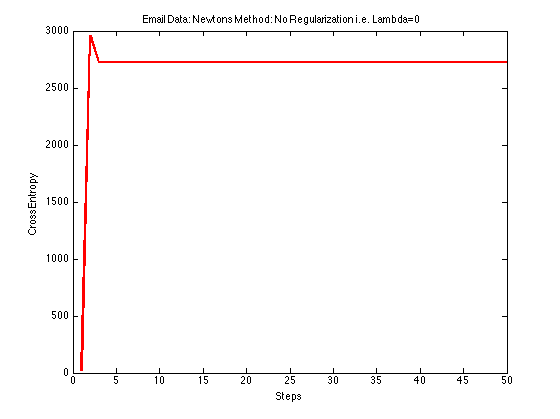
\includegraphics[width=0.8\textwidth]{../Pics/newton/email_unreg.png}
\end{figure}

\begin{figure}[h!]
  \caption{Cross-Entropy wrt Steps: Email Train Data Regularized}
  \centering
    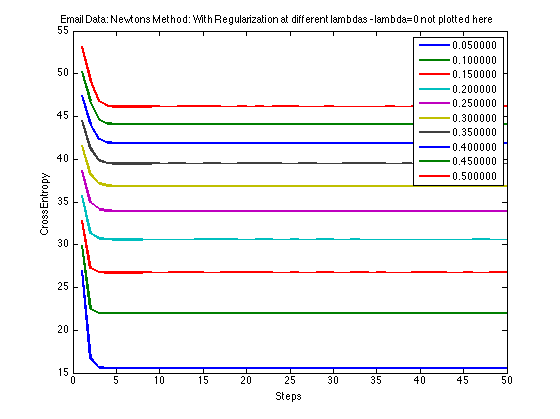
\includegraphics[width=0.8\textwidth]{../Pics/newton/email_reg.png}
\end{figure}


\begin{figure}[h!]
  \caption{Cross-Entropy wrt Steps: Ionosphere Train Data Unregularized}
  \centering
    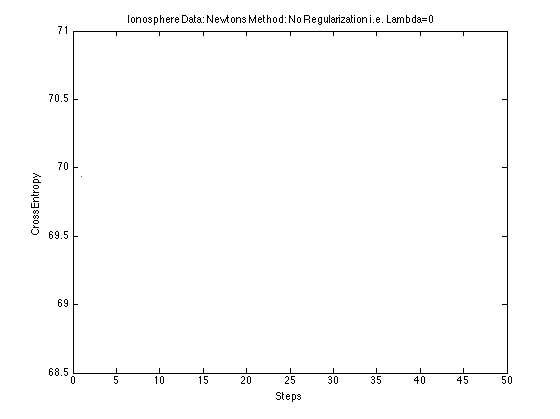
\includegraphics[width=0.8\textwidth]{../Pics/newton/iono_unreg.png}
\end{figure}



\begin{figure}[h!]
  \caption{Cross-Entropy wrt Steps: Ionosphere Train Data Regularized}
  \centering
    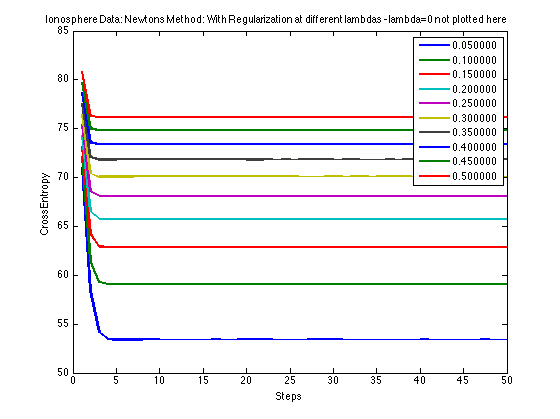
\includegraphics[width=0.8\textwidth]{../Pics/newton/iono_reg_full.png}
\end{figure}



\end{document}